\chapter{The Effect of Ebola Glycoprotein Evolution on Protein Flexibility}
CA Mirabzadeh

%\section*{Abstract}

\section{Introduction}

The 2014 Ebola epidemic has provided a wealth of information that can be used to understand Ebola evolution and how it could modify the efficacy of vaccines. The goal of this study is to determine the effects of previous, ongoing, and future viral evolution on the structure and antibody binding properties of Ebola glycoprotein (GP). Our focus is on the disordered mucin-like domain of GP. Analysis suggests that, while most of the disordered region of GP is evolving in a neutral fashion \cite{Olabode2015, Li2014}, a few sites are undergoing positive selection, FIG. \ref{ebolagp}.

\section{Methods}
Molecular dynamics simulations were performed using the GROMACS \cite{Berendsen1995} simulation package. Neutral capping was used to ensure there were no electrostatic interactions between the ends of the peptides. Simulated tempering was used to increase the exploration of conformational space. Simulations were initiated with fully extended peptide conformations generated using the Python package PMX  \cite{Gapsys2015}.

\section{Results Discussion and Conclusion}

In order to understand selection relative to the flexibility of mutations we focused on positively selected sites, (Table \ref{possites}), in the disordered mucin-like domain of the Ebola virus glycoprotein.  We looked at flexibility, FIG. \ref{avgrms}, by averaging the root mean square deviation over five separate simulations of the disordered sites with positively selected peptides. In the future we would like to look at the entire mucin-like domain and see how multiple mutations work together to change flexibility.

\begin{table}[ht]
\caption{Positively selected sites. Three pairs of sequences from human sources used for our analysis. The first of each pair is a representative of a current sequence. The second simply has the ancestral amino acid inserted at the center position. The Democratic Republic of the Congo (DRC) is a country located in Central Africa. From 1971 to 1997 it was named Zaire.}
\centering
\begin{tabular}{ccc}
\hline \\
Residue & Sequence & Origin \\
\hline \\
L at 442 & SKGTDLLDPAT & Zaire 1995 \\
Ancestor at 442 & SKGTDFLDPAT & \\
S at 442 & SKSADSLDLAT & DRC 2014 \\
Ancestor at 442 & SKSADFLDLAT & \\
L at 429 & TAAGPLKAENT & Zaire 1995 \\
Ancestor at 429 & TAAGPPKAENT & \\
P at 376 & STSPQPPTTKT & DRC 2014 \\
Ancestor at 376 & STSPQSPTTKT &  \\
\hline \\
\end{tabular}
\label{possites}
\end{table}

\section{Acknowledgments}

Grant support for this research was provided by the National Science Foundation (DEB1521049) and the Center for Modeling Complex Interactions sponsored by the National Institutes of Health (P20 GM104420). Computer resources were provided in part by the Institute for Bioinformatics and Evolutionary Studies Computational Resources Core sponsored by the National Institutes of Health (P30 GM103324).


\begin{figure*}[htbp]
    \centering
    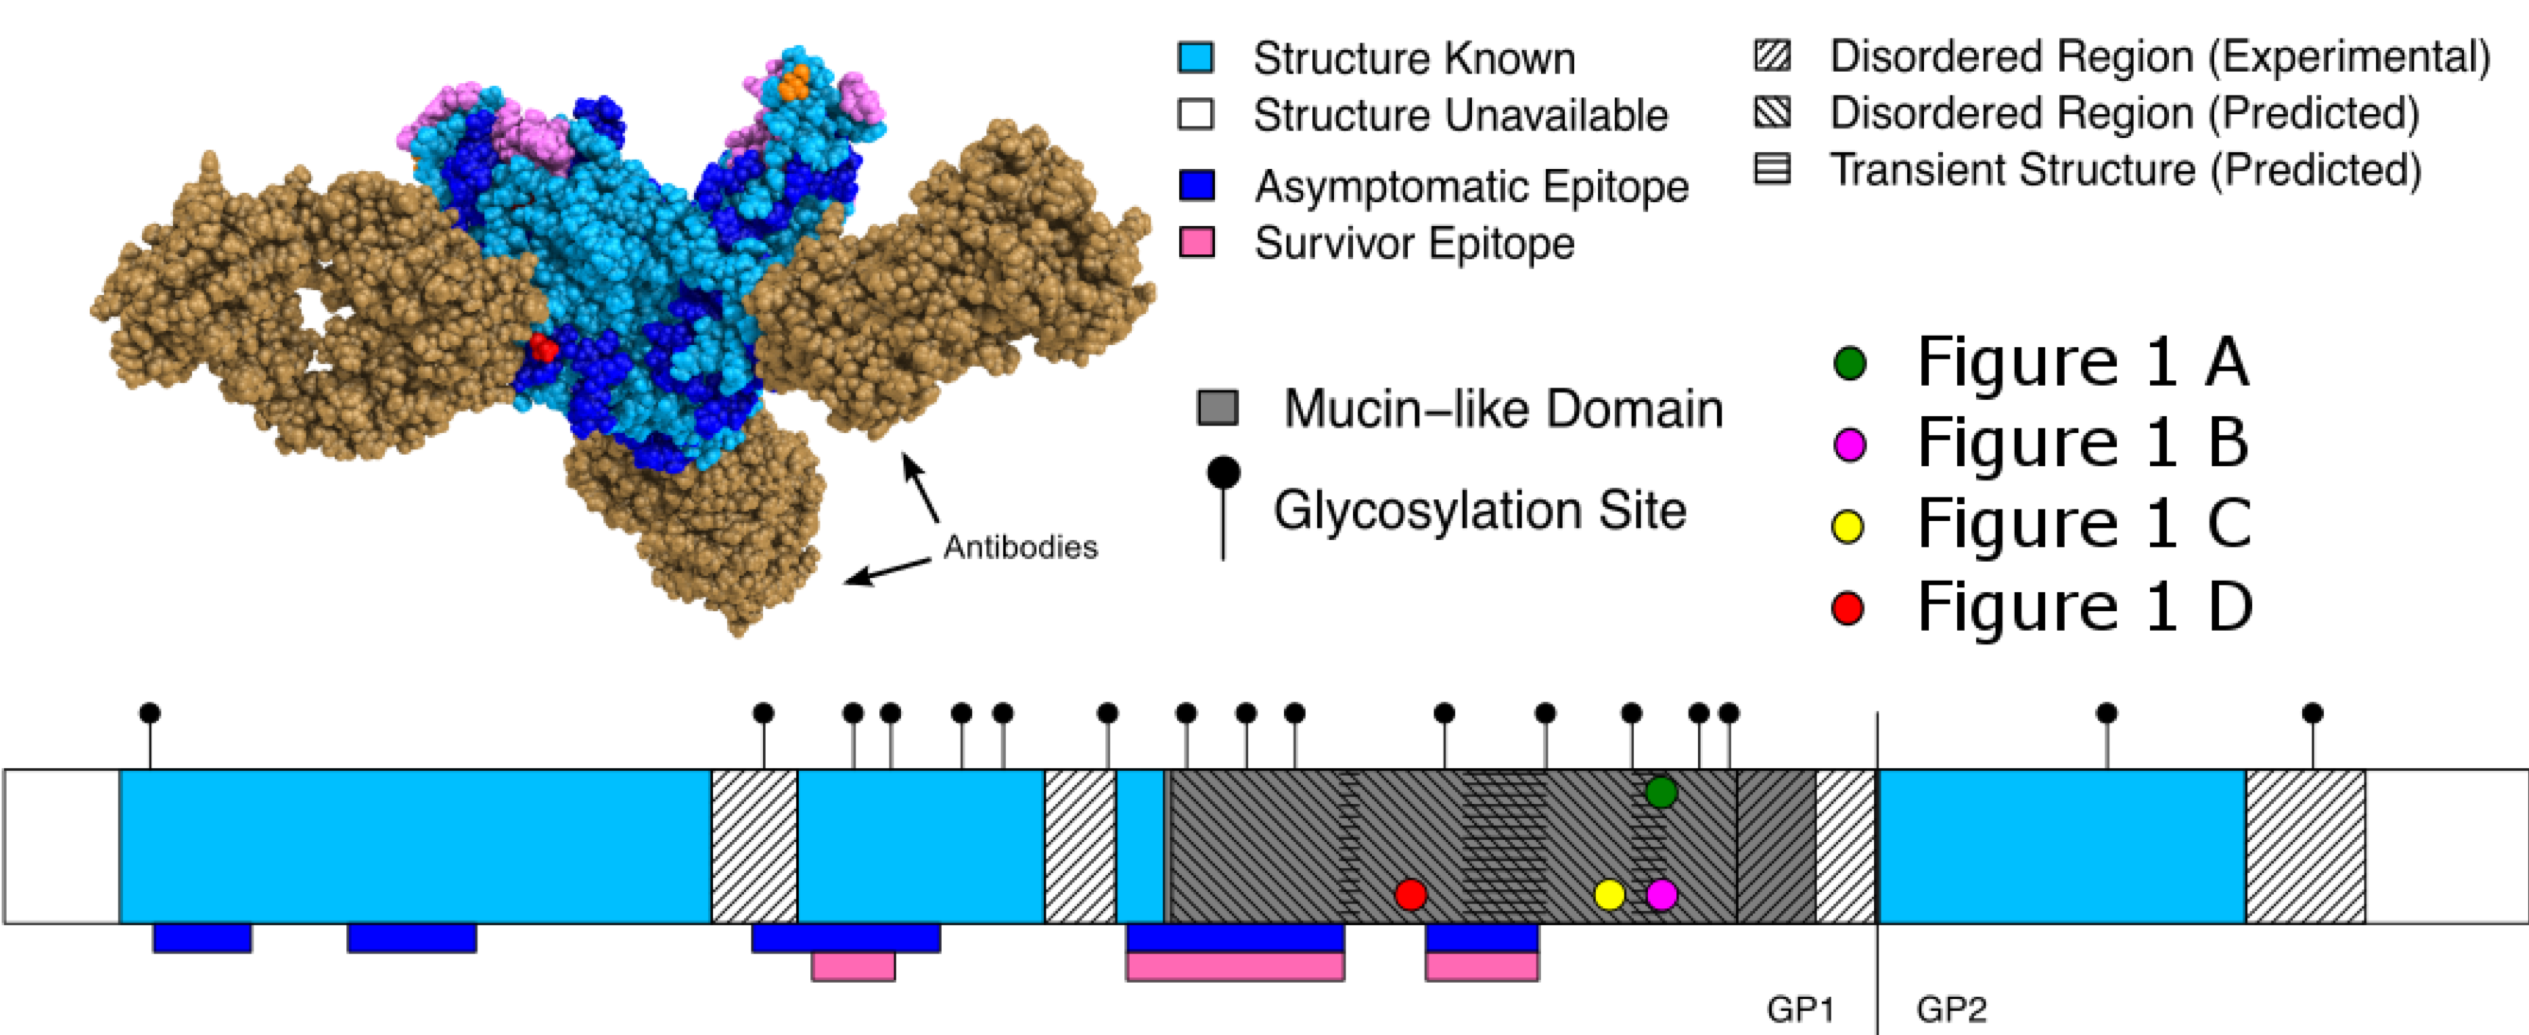
\includegraphics[width=1 \textwidth]{figures/ebolagraphic002.png}
    \caption{The Ebola glycoprotein. The positively selected sites are in the mucin-like domain. Evolutionary analysis results show that there has been some evolution that may change the way that antibodies bind to GP.}
    \label{ebolagp}
\end{figure*}

\begin{figure*}[htbp]
    \centering
    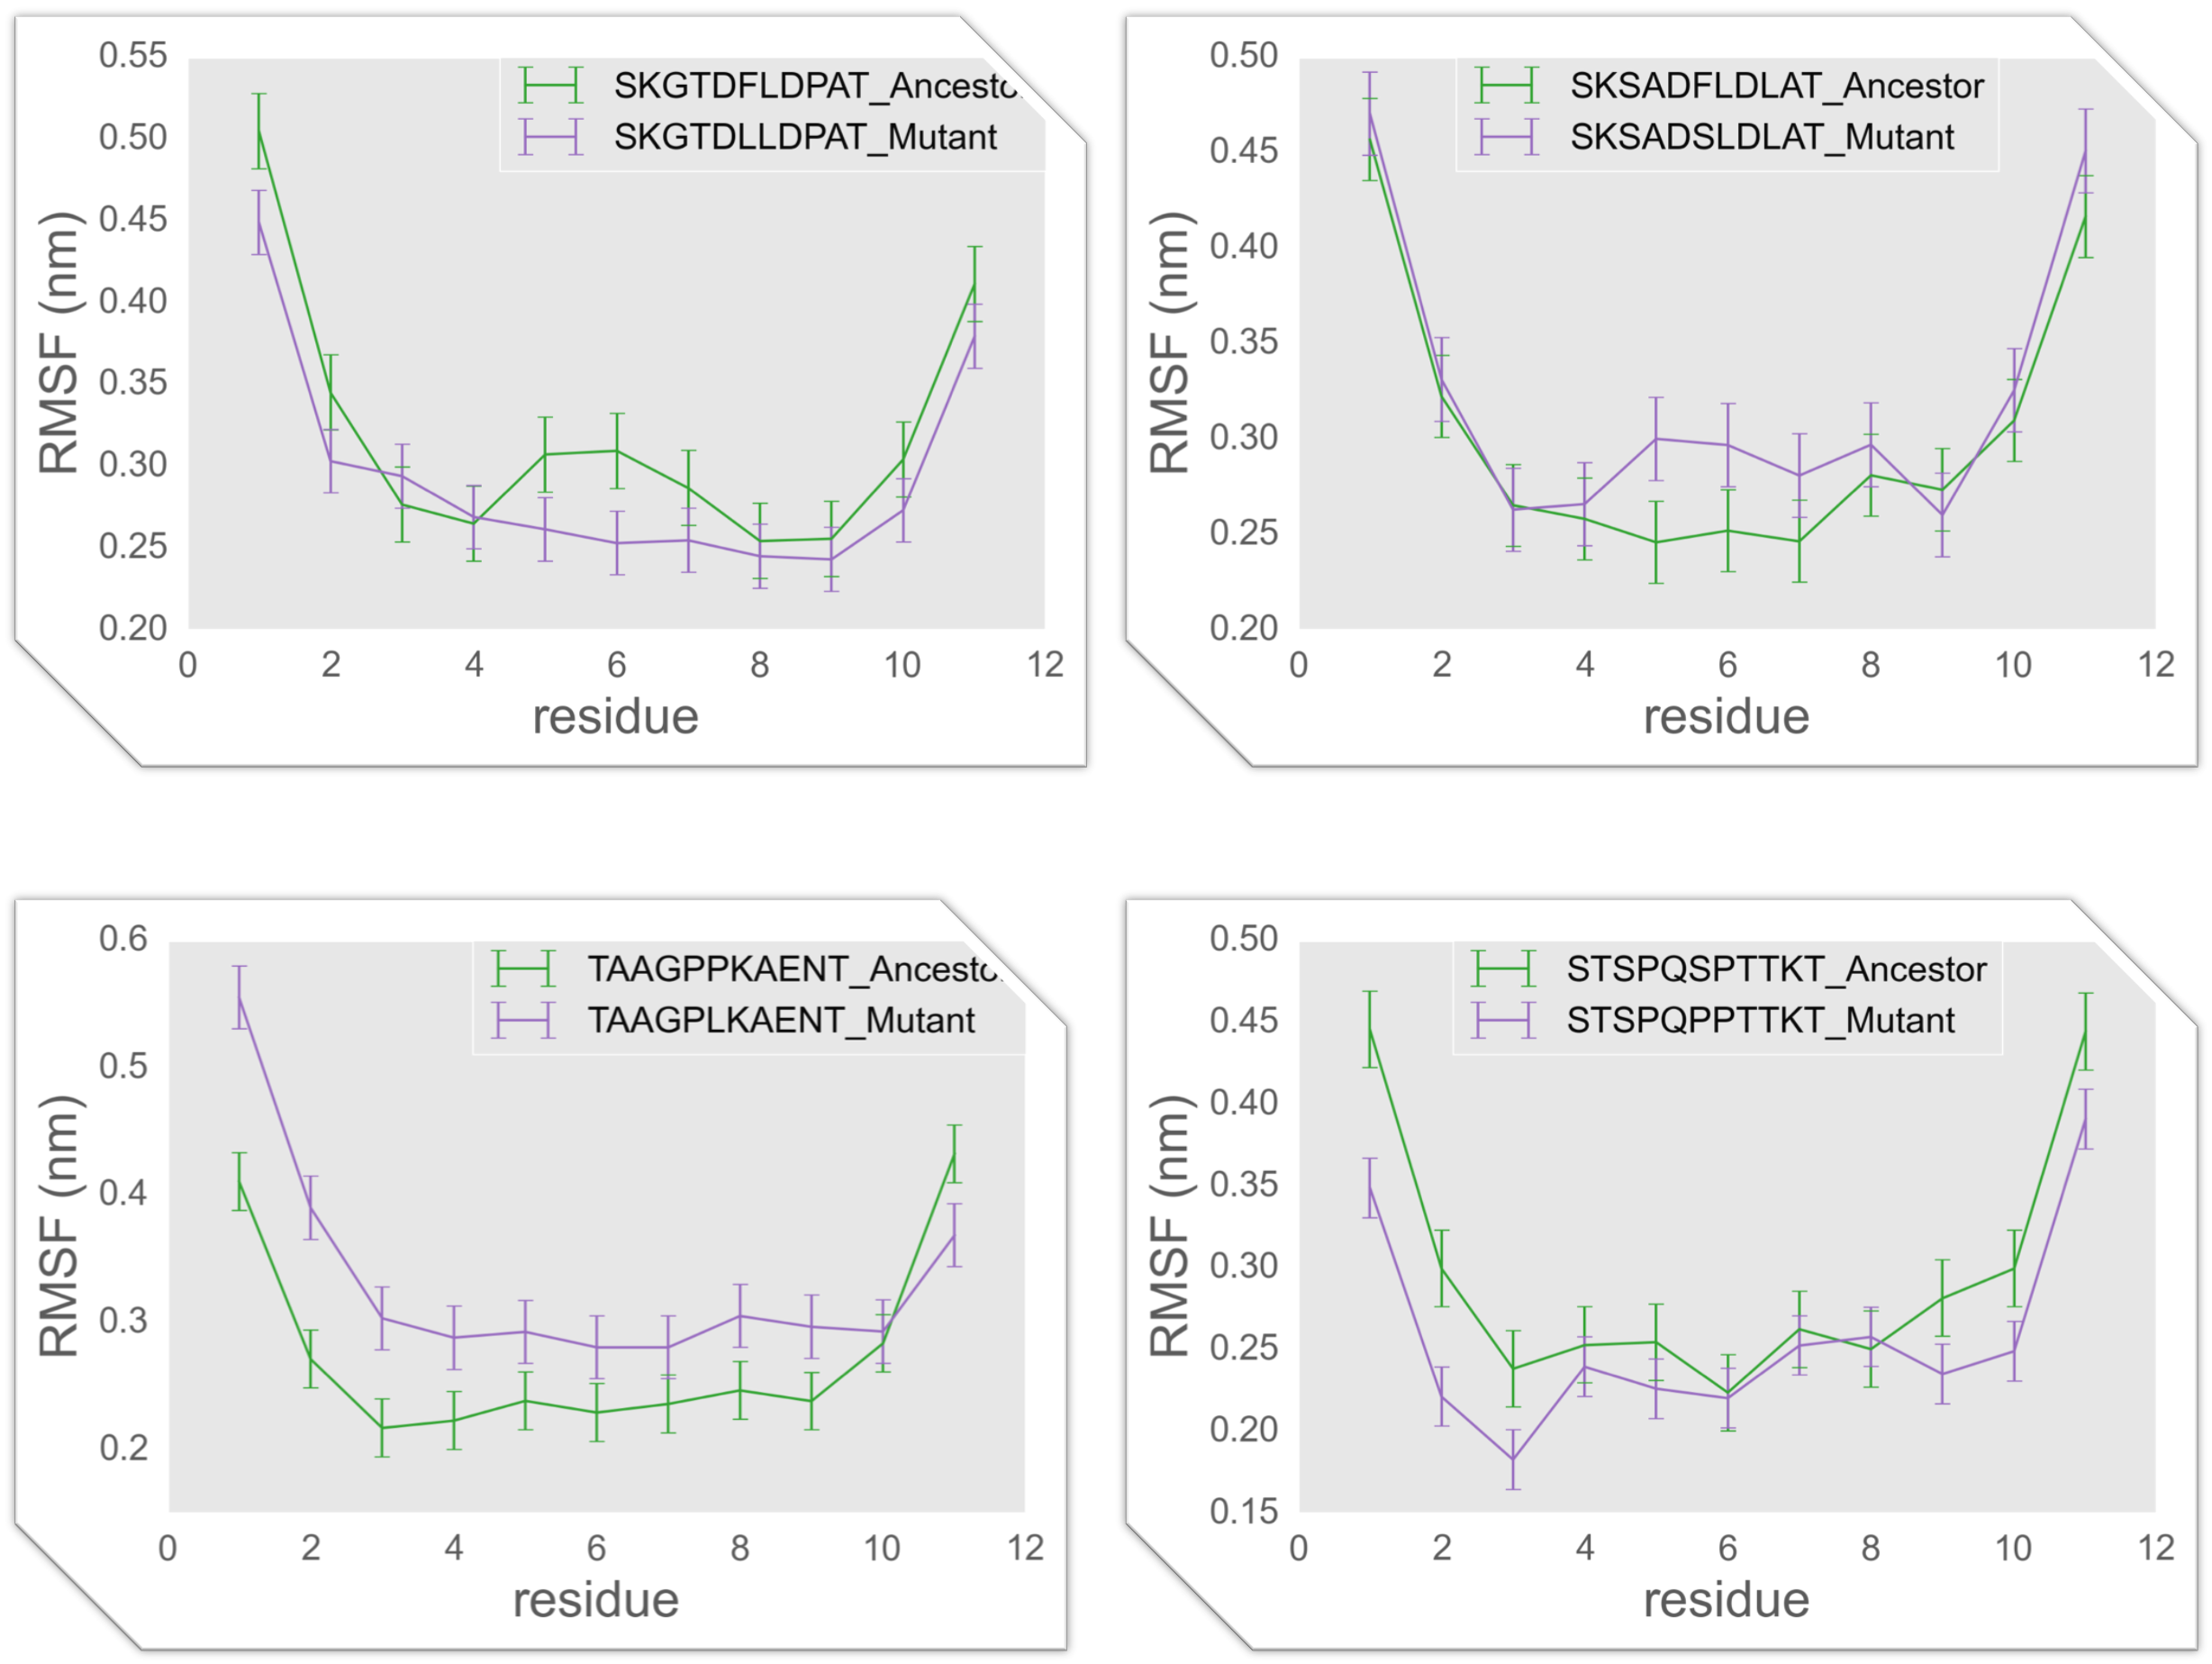
\includegraphics[width=1\textwidth]{figures/ebolagraphic001.png}
    \caption{Average C-alpha Root Mean Square Fluctuation. To understand the biophysical implications of mutations in the Ebola glycoprotein mucin-like domain, we performed molecular dynamics simulations of small fragments of the protein. The Root Mean Square Fluctuation was averaged over five separate time evolution simulations for each peptide.}
    \label{avgrms}
\end{figure*}